% ----- Consignes exo 1 ----- %
\begin{td-exo}[Echauffement]\,\\ % 1
    Calculer la sommet-connectivité et l'arête-connectivité du graphe suivant:

    \vspace{0.2cm}
    \input{../assets/tikz/td_4_ex_1_1.tex}
\end{td-exo}

% ----- Solutions exo 1 ----- %
\iftoggle{showsolutions}{
	\begin{td-sol}[]\,\\ % 1
		On peut remarquer que la partie centrale du graph est surement la plus facile à séparer du reste du graphe.
        On peut alors voir que la sommet-connectivité est de \(2\) en enlevant les sommets \(g\) et \(h\), et 
        que l'arête-connectivité est de \(3\) en enlevant les arêtes \(\{(e, g), (c, h), (f, h)\}\):

        \vspace{0.2cm}
        \begin{figure}[H]
            \CenterFloatBoxes{}
            \begin{floatrow}
                % Figure BFS 1
\ffigbox[\FBwidth]{
\caption{\centering Graphe \(G\) privé \\des sommets \(g\) et \(h\)}\label{Fig:td_4_ex_1_2}
}{
    \fbox{
        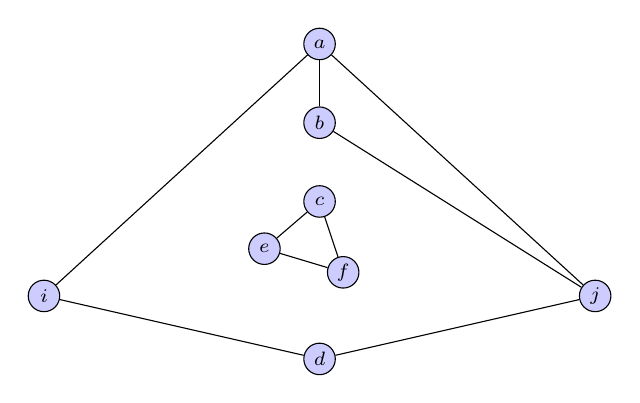
\begin{tikzpicture}[scale=1, every node/.style={circle, draw, fill=blue!20, inner sep=1pt, font=\scriptsize, minimum size=4mm}]
            \node (a) at (0, 2) {\(a\)};
            \node (b) at (0, 1) {\(b\)};
            \node (c) at (0, 0) {\(c\)};
            \node (d) at (0, -2) {\(d\)};

            \node (e) at (-0.7, -0.6) {\(e\)};
            \node (f) at (0.3, -0.9) {\(f\)};

            % \node (g) at (-2, -0.6) {\(g\)};
            % \node (h) at (2, -0.6) {\(h\)};

            \node (i) at (-3.5, -1.2) {\(i\)};
            \node (j) at (3.5, -1.2) {\(j\)};

            \draw (a) -- (b);
            % \draw (a) -- (g);
            \draw (a) -- (i);
            \draw (a) -- (j);

            % \draw (b) -- (g);
            % \draw (b) -- (h);
            \draw (b) -- (j);

            \draw (c) -- (e);
            \draw (c) -- (f);
            % \draw (c) -- (h);

            % \draw (d) -- (g);
            % \draw (d) -- (h);
            \draw (d) -- (i);
            \draw (d) -- (j);

            \draw (e) -- (f);
            % \draw (e) -- (g);

            % \draw (f) -- (h);

            % \draw (g) -- (i);

            % \draw (h) -- (j);
        \end{tikzpicture}
    }
}

                % Figure BFS 1
\ffigbox[\FBwidth]{
\caption{\centering Graphe \(G\) privé \\des arêtes \(\{(e, g), (c, h), (f, h)\}\)}\label{Fig:td_4_ex_1_3}
}{
    \fbox{
        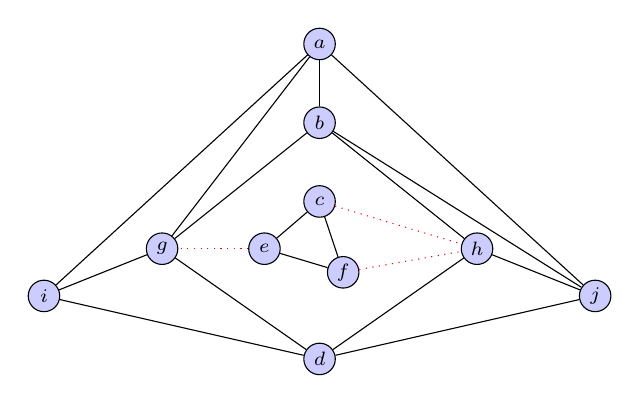
\begin{tikzpicture}[scale=1, every node/.style={circle, draw, fill=blue!20, inner sep=1pt, font=\scriptsize, minimum size=4mm}]
            \node (a) at (0, 2) {\(a\)};
            \node (b) at (0, 1) {\(b\)};
            \node (c) at (0, 0) {\(c\)};
            \node (d) at (0, -2) {\(d\)};

            \node (e) at (-0.7, -0.6) {\(e\)};
            \node (f) at (0.3, -0.9) {\(f\)};

            \node (g) at (-2, -0.6) {\(g\)};
            \node (h) at (2, -0.6) {\(h\)};

            \node (i) at (-3.5, -1.2) {\(i\)};
            \node (j) at (3.5, -1.2) {\(j\)};

            \draw (a) -- (b);
            \draw (a) -- (g);
            \draw (a) -- (i);
            \draw (a) -- (j);

            \draw (b) -- (g);
            \draw (b) -- (h);
            \draw (b) -- (j);

            \draw (c) -- (e);
            \draw (c) -- (f);
            \draw[dotted, draw=red] (c) -- (h);

            \draw (d) -- (g);
            \draw (d) -- (h);
            \draw (d) -- (i);
            \draw (d) -- (j);

            \draw (e) -- (f);
            \draw[dotted, draw=red] (e) -- (g);

            \draw[dotted, draw=red] (f) -- (h);

            \draw (g) -- (i);

            \draw (h) -- (j);
        \end{tikzpicture}
    }
}
            \end{floatrow}
        \end{figure}

        Il n'y a pas de méthode simple pour prouver ce résultat, pour la sommet-connectivité on peut noter qu'il existe un cycle hamiltonien dans le graphe \(G\) de départ, donc la sommet-connectivité est au moins de \(2\).

        Pour la sommet-connectivité il n'existe pas de méthode simple non plus, on peut juste montrer que toute paire d'arêtes ne sépare pas le graphe en deux composantes connexes.
	\end{td-sol}
}{}


% ----- Consignes exo 2 ----- %
\begin{td-exo}[Echauffement (plus dur)]\,\\ % 2
    Calculer \(\kappa(P)\) (où \(P\) est le graphe de Petersen), \(\lambda(K_n)\) (où \(K_n\) est le graphe complet à \(n\) sommets; on pourra utiliser le fait que si \(F\) est un ensemble d'arêtes de taille \(\leq n-2\) de \(K_n\), alors\(V(K_n), F\) n'est pas connexe), et \(\kappa(Q_d)\) (où \(Q_d\) est le graphe hypercube de dimension \(d\), de sommets \({\left\{0,1\right\}}^d\) avec \(x_1, \ldots, x_d\) et \(y_1, \ldots ,y_d\) reliés si et seulement si \(\sum_{i=1}^d |x_i - y_i| = 1\); on pourra raisonner par récurrence sur \(d\)).
\end{td-exo}

% ----- Solutions exo 2 ----- %
\iftoggle{showsolutions}{
	\begin{td-sol}[]\, % 2
		\begin{enumerate}
            \item On peut constater graphiquement que \(\kappa(P) = 3\).

            \item Soit \(F\) un arête-séparateur minimum de \(K_n\).
            Si \(|F| \leq n-2\), alors \((V(K_n), F)\) n'est pas connexe.
            Il admet donc une partition \((C,V \setminus C)\) sans arête entre les deux parties.

            Donc \(K_n \setminus F\) contient toutes les arêtes entre \(C\) et \(V \setminus C\), donc il est connexe, ce qui est absurde.
            Donc \(|F| \geq n-1\).
        \end{enumerate}
	\end{td-sol}
}{}


% ----- Consignes exo 3 ----- %
\begin{td-exo}[Connectivité des cubiques]\,\\ % 3
    Trouver un graphe \(G\) vérifiant \(\lambda(G) = 3\) et \(\kappa(G) = 1\).

    Soit \(G\) un graphe cubique (i.e. \(3\)-régulier). Montrer que \(G\) est \(3\)-arête-connexe si et seulement si il est \(3\)-sommet-connexe.
\end{td-exo}

% ----- Solutions exo 3 ----- %
\iftoggle{showsolutions}{
	\begin{td-sol}[]\,\\ % 3
		On peut même résoudre ce problème pour \(\lambda(G) = n\) avec le graphe suivant:

        \vspace{0.2cm}
        % Figure BFS 1
\ffigbox[\FBwidth]{
\caption{\centering Graphe \(G\) vérifiant \\\(\lambda(G) = n\) et \(\kappa(G) = 1\)}\label{Fig:td_4_ex_3_1}
}{
    \fbox{
       \begin{tikzpicture}[scale=1, main node/.style={circle, draw, fill=blue!20, inner sep=1pt, font=\scriptsize, minimum size=6mm}]
            % les sommets de X
            \node[main node] (x1) at (-2, 2) {\(x_1\)};
            \node[] (xdots1) at (-1, 2) {\(\cdots\)};
            \node[] (xdots2) at (0, 2) {\(\cdots\)};
            \node[] (xdots3) at (1, 2) {\(\cdots\)};
            \node[main node] (xn) at (2, 2) {\(x_n\)};

            % les sommets de Y
            \node[main node] (y1) at (-2, -2) {\(y_1\)};
            \node[] (ydots1) at (-1, -2) {\(\cdots\)};
            \node[] (ydots2) at (0, -2) {\(\cdots\)};
            \node[] (ydots3) at (1, -2) {\(\cdots\)};
            \node[main node] (yn) at (2, -2) {\(y_n\)};

            % le sommet central
            \node[main node] (c) at (0, 0) {\(c\)};
            
            % on entoure X
            \node[inner sep=12pt, fit=(x1) (xn), name=XFIT] {};
            \node[inner sep=12pt, fit=(y1) (yn), name=YFIT] {};

            \draw[green!60, thick, fill=green!20, opacity=0.4, rotate around={90:(XFIT.center)}]
                (XFIT.center) ellipse [x radius=0.8cm, y radius=2.5cm];
            \node at (XFIT.north) [yshift=11pt] {\(X = K_n\)};

            \draw[green!60, thick, fill=green!20, opacity=0.4, rotate around={90:(YFIT.center)}]
                (YFIT.center) ellipse [x radius=0.8cm, y radius=2.5cm];
            \node at (YFIT.south) [yshift=-11pt] {\(Y = K_n\)};
            % les aretes entre X et c
            \draw (x1) -- (c);
            \draw[dotted] (xdots1) -- (c);
            \draw[dotted] (xdots2) -- (c);
            \draw[dotted] (xdots3) -- (c);
            \draw (xn) -- (c);

            % les aretes entre Y et c
            \draw (y1) -- (c);
            \draw[dotted] (ydots1) -- (c);
            \draw[dotted] (ydots2) -- (c);
            \draw[dotted] (ydots3) -- (c);
            \draw (yn) -- (c);
        \end{tikzpicture}
    }
}

        On voit alors clairement que chaque composante \(X\) et \(Y\), étant un graphe complet à \(n\) sommets est \(n\) régulier (car chaque sommet est aussi relié au sommet central \(c\)). Ainsi il faut enlever au moins \(n\) arêtes pour séparer un sommet de \(G\) mais en enlevant le sommet \(c\) on sépare le graphe en deux composantes connexes, donc \(\kappa(G) = 1\) et \(\lambda(G) = n\).

        Par le cours, on a
        \begin{equation*}
            \kappa(G) \leq \lambda(G) \leq \delta(G) = 3
        \end{equation*}
        donc le sens direct est évident, \(\kappa(G) = 3 \implies \lambda(G) = 3\).

        Inversement, supposons que \(\lambda(G) = 3\) et traitons les cas:
        \begin{itemize}
            \item On a \(\kappa > 0\) car \(G\) est connexe.

            \item Si \(\kappa(G) = 1\), alors il existe un sommet \(x\) tel que \(G \setminus \{x\}\) est déconnecté.
            Alors \(G \setminus x\) possède une partition \((C, V \setminus C)\) telle qu'il n'existe pas d'arête entre \(C\) et \(V \setminus C\).

            Sans perte de généralité, supposons que \(x\) a un voisin dans \(C\) et deux dans \(V \setminus C\).

            Alors, en enlevant l'arête entre \(x\) et \(C\), le graphe n'est plus connexe, ce qui est absurde (car \(\lambda(G) = 3\)).

            \item Si \(\kappa(G) = 2\), alors il existe deux sommets \(x,y\) tels que \(G \setminus \{x,y\}\) est déconnecté.
            Alors \(G \setminus \{x,y\}\) possède une partition \((C, V \setminus C)\) telle qu'il n'existe pas d'arête entre \(C\) et \(V \setminus C\).
            % insert nice graph here

            Sans perte de généralité, supposons que \(x\) a un voisin dans \(C\) (sinon \(y\) sépare \(C\) de \(V \setminus C \cup \{x\}\), ce qui est absurde).

            De même, \(x\) possède un voisin dans \(V \setminus C\) (sinon \(y\) sépare \(C \cup \{x\}\) de \(V \setminus C\), ce qui est absurde). Donc \(x\) possède un voisin dans chaque partie.

            De même, \(y\) possède un voisin dans chaque partie.

            Pour que \(\{xx_C, y y_C\}\) ne soit pas un arête-séparateur, il faut une arête de plus entre \(C\) et \(\{x,y\}\).
            De même, pour que \(\{x x_{V \setminus C}, y y_{V \setminus C}\}\) ne soit pas un arête-séparateur, il faut une arête de plus entre \(V \setminus C\) et \(\{x,y\}\). Alors, en enlevant les arêtes \(x x_{C'}, y y_{C}\) on a bien trouvé un arête-séparateur de taille \(2\), ce qui est absurde.

            \item Donc \(\kappa(G) \geq 3\). Comme \(\kappa(G) \leq \lambda(G) = 3\), on a bien \(\kappa(G) = 3\).
        \end{itemize}
	\end{td-sol}
}{}


% ----- Consignes exo 4 ----- %
\begin{td-exo}[Treillis des séparateurs]\,\\ % 4
    Soient \(G = (V,E)\) un graphe connexe et \(x,y\) deux sommets de \(G\).
    Pour \(X\) un \((x,y)\)-(sommet-)séparateur de \(G\), on note \(C(X,x)\) la composante connexe de \(G\setminus X\) contenant \(x\). % chktex 36

    Soient \(X\) et \(Y\) deux \((x,y)\)-(sommets-)séparateurs, montrer que \(A = (X \cap C(Y,x)) \cup (X \cap Y) \cup (Y \cap C(X,x))\) et \(B = (X \cap C(Y,y)) \cup (X \cap Y) \cup (Y \cap C(X,y))\) sont aussi des \((x,y)\)-(sommets-)séparateurs de \(G\). % chktex 36 % chktex 10
\end{td-exo}

% ----- Solutions exo 4 ----- %
\iftoggle{showsolutions}{
	\begin{td-sol}[]\,\\ % 4
		Exercice solution
	\end{td-sol}
}{}


% ----- Consignes exo 5 ----- %
\begin{td-exo}[Graphes \(2\)-connexes]\,\\ % 5
    Exercise 5 content
\end{td-exo}

% ----- Solutions exo 5 ----- %
\iftoggle{showsolutions}{
	\begin{td-sol}[]\,\\ % 5
		Exercice solution
	\end{td-sol}
}{}


% ----- Consignes exo 6 ----- %
\begin{td-exo}[Menger étendu]\,\\ % 6
    Exercise 6 content
\end{td-exo}

% ----- Solutions exo 6 ----- %
\iftoggle{showsolutions}{
	\begin{td-sol}[]\,\\ % 6
		Exercice solution
	\end{td-sol}
}{}


% ----- Consignes exo 7 ----- %
\begin{td-exo}[Plein de cycles]\,\\ % 7
    Exercise 7 content
\end{td-exo}

% ----- Solutions exo 7 ----- %
\iftoggle{showsolutions}{
	\begin{td-sol}[]\,\\ % 7
		Exercice solution
	\end{td-sol}
}{}


% ----- Consignes exo 8 ----- %
\begin{td-exo}[Gros cycle]\,\\ % 8
    Exercise 8 content
\end{td-exo}

% ----- Solutions exo 8 ----- %
\iftoggle{showsolutions}{
	\begin{td-sol}[]\,\\ % 8
		Exercice solution
	\end{td-sol}
}{}


% ----- Consignes exo 9 ----- %
\begin{td-exo}[Arbres couvrants disjoints]\,\\ % 9
    Exercise 9 content
\end{td-exo}

% ----- Solutions exo 9 ----- %
\iftoggle{showsolutions}{
	\begin{td-sol}[]\,\\ % 9
		Exercice solution
	\end{td-sol}
}{}


% ----- Consignes exo 10 ----- %
\begin{td-exo}[Pas plus de deux\(\ldots\)]\,\\ % 10
    Exercise 10 content
\end{td-exo}

% ----- Solutions exo 10 ----- %
\iftoggle{showsolutions}{
	\begin{td-sol}[]\,\\ % 10
		Exercice solution
	\end{td-sol}
}{}


% ----- Consignes exo 11 ----- %
\begin{td-exo}[Jeu de Shannon]\,\\ % 11
    Exercise 11 content
\end{td-exo}

% ----- Solutions exo 11 ----- %
\iftoggle{showsolutions}{
	\begin{td-sol}[]\,\\ % 11
		Exercice solution
	\end{td-sol}
}{}

